\documentclass[journal,twoside]{JoPhA}

\usepackage{color}
\usepackage{flushend}
\usepackage{fancyvrb}
\usepackage[pdftex]{graphicx}
\usepackage{hyperref}


% declare the path(s) where your graphic files are
\graphicspath{{figures/}}
% and their extensions so you won't have to specify these with
% every instance of \includegraphics
\DeclareGraphicsExtensions{.pdf,.jpeg,.png}


\begin{document}

\title{Cybersecurity in Autonomous Systems: Evaluating the performance of hardened ROS}

\author{Francisco Javier Rodr\'iguez Lera, Jes\'us Balsa, Fernando Casado, Camino Fern\'andez, Francisco Mart\'in Rico, and Vicente Matell\'an
\IEEEcompsocitemizethanks{
Francisco Javier Rodr\'iguez Lera, Jes\'us Balsa, Fernando Casado, Camino Fern\'andez, and Vicente Matell\'an are with the Robotics Group (http://robotica.unileon.es) and the Research Institute on Applied Sciences to Cybersecurity (http://riasc.unileon.es) at Universidad de Le\'on (Spain).

Francisco Martín Rico is with Robotics Lab, Signal Theory, Communications, Telematic Systems and Computation Department at Universidad Rey Juan Carlos, Madrid (Spain).

\IEEEcompsocthanksitem Corresponding author: vicente.matellan@unileon.es}% <-this % is needed.
}






\markboth{Workshop on Physical Agents, M\'alaga 2016}%
{Matell\'an et al: Cybersecurity in ROS}
\maketitle


\begin{abstract}
As robotic systems spread, cybersecurity emerges as major concern. Currently most research autonomous systems are built using the ROS framework, along with other commercial software. 
ROS is a distributed framework where nodes publish information that other nodes consume. 
This model simplifies data communication but poses a major threat because a malicious process could easily interfere the communications, read private messages or even supersede nodes. In this paper we propose that ROS communications should be encrypted. We also measure how encryption affects its performance. We have used three different ciphering techniques: DES, AES and RSA. We have evaluated the performance of the system, both from the computing and the communications point of view. Preliminary results show that symmetric ciphers using private keys impose significant delays.
\end{abstract}


\begin{IEEEkeywords}
Autonomous systems, Cybersecurity, Data security, Cyber-physical systems, ROS, Performance analysis
\end{IEEEkeywords}


\section{Introduction}


% \IEEEPARstart{A}{utonomous} systems are spreading not just in the virtual world (Internet, software systems), or in science-fiction movies, but in our ordinary real world. 
\IEEEPARstart{I}{t} is possible to find driverless cars in the streets, autonomous vacuum cleaners in our homes, autonomous robotic guides at museums, etc. These robotic systems, as any computer-based system, can suffer different types of cyber-attacks, and some degree of cybersecurity \cite{Morante2015} is required. 


Our research group is developing an assistant robot~\cite{Martin2014} for the elderly. When we initiated experiments involving potential users, caregivers asked us about the security of our robot and about the privacy of its communications \cite{Denning2009}. When an assistant robot carrying a camera is deployed in a home, the access to this camera should be secured; even more when the robot is managing medical information. 

We have developed all the software that controls the autonomous behavior of our robot using ROS (Robotic Operating System) \cite{ROS09} which has become the most popular framework for developing robotic applications. It started as a research framework, but currently most of manufacturers of commercial platforms use ROS as the {\em de facto} standard for building robotic software. For example, object-manipulation robots like Baxter (by Rethink robotics) ~\cite{fitzgerald2013developing} or service robots as our RB1 (by Robotnik) are ROS based platforms.

%We realized that the communication mechanism was one of its weakest points. 

%Some works have been sketched in this area, as for instance in \cite{Guiochet2016}.



\subsection{Security assessment}


There are three basic vulnerabilities threatening any computer system: availability (data interruption), confidentiality (data interception) and integrity (data modification). Other authors also add two more~\cite{sattarova2007security}: authenticity and non-repudiation (data fabrication from a non-trusted origin). 

These concepts can be easily translated to industrial control applications~\cite{huitsing2008attack} or to robotic environments, due to the distributed approach used in most extended robotic frameworks (Yarp, ROS, ROBOCOMP). On one hand, the robot is deployed in a home environment. The robot provides information to users and also carries out behaviors in order to fulfill required tasks. 

On the other hand, an attacker could attempt to make the robot or its network resources unavailable, this is a denial-of-service attack. The attacker could also intercept and modify command messages in order to change robot behavior, and capture robot information about the environment and about the users. Finally the attacker could simulate a sensor and generate new data and send it to the robot. Fig. \ref{fig:Conceptualmodel} summarizes graphically these vulnerabilities in a robotic environment.

\begin{figure}[ht]
	\centering
	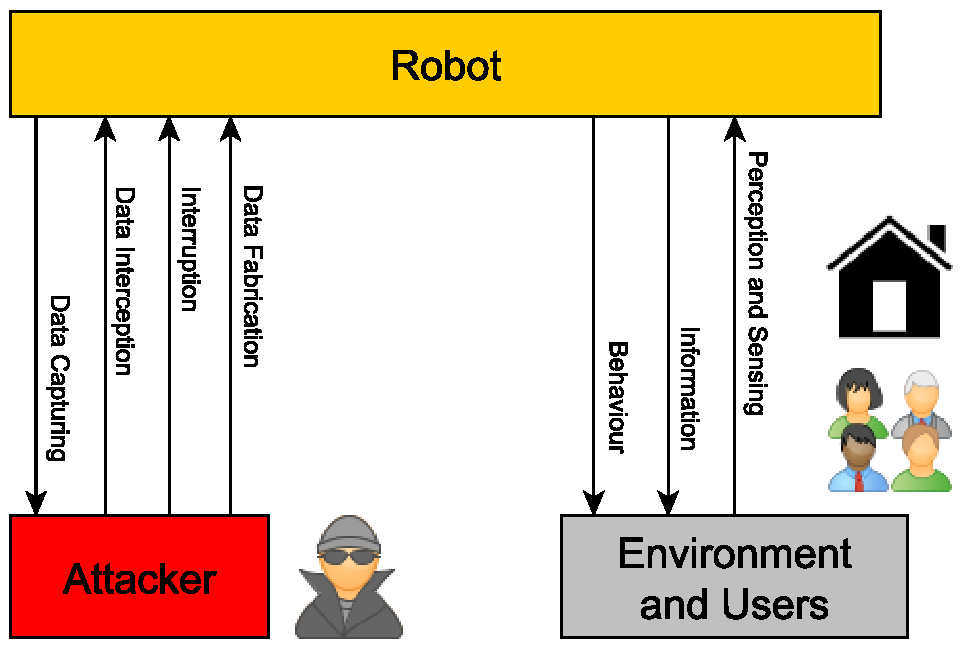
\includegraphics[width=.5\textwidth]{RobotsAttacks.pdf}
	\caption{Conceptual model of the security attacks.}
	\label{fig:Conceptualmodel}
\end{figure}

In this research we focus on confidentiality of data sent to and from the robot. Our proposal consists in encrypt data transmitted between ROS processes, adding two nodes for encryption and decryption task. We don't change ROS messages nor ROS standard functions to send the data. The question is if this hardening of ROS will impact on its performance.



The reminder of this paper is organized as follows: Next section describes the ROS framework communication process. Section~\ref{Description} defines the testbed designed to measure the performance of the encrypted ROS system. Section~\ref{experiments} shows the data obtained in the proposed experiments as well as the discussion. Finally section\ref{conclusions} presents the conclusions obtained and further work.

% \begin{enumerate}
%  \item Availability: Interruption
%  \item Confidenciatily: Interception
%  \item Integrity: Modification
%  \item Authenticity: Fabrication
% \end{enumerate}



\section{ROS overview}
\label{ROS_overview}
ROS provides specific libraries for robotics as well as classical operating system services such as hardware abstraction (for sensors and actuators), low-level device control, and inter-process communication. Inter-process communication is based on a graph architecture where computation takes place in ROS processes named nodes. These nodes can receive and send messages, but no security was considered in the communication mechanism.

ROS framework is basically a message-passing distributed system. Its architecture is based on processes that publish {\em messages} to {\em topics}. For instance, a process ({\em node}) can be in charge of accessing a sensor, performing the information processing, and publishing it as an information structure on a named topic. Another process can {\em subscribe} to this topic, that is, read its information. Then the process can make a decision about the movement of the robot. Next, this node will publish the commands in another topic to send them to the motors. ROS nodes can be running in the same computer or in different computers.

Conventional ROS environment is composed by at least one ROS Master and some clients. ROS Master is the key element in the ROS system. It runs as a nameservice and manages registration information of topics and services used by ROS nodes. 

When a node wants to stablish a connection with a topic, it communicates with Master to advise its registration information. After this step, the node gets more information about other registered nodes so it can stablish new connections with their topics appropriately. The Master is updated in real time with nodes information and topics they publish/subscribe. Fig.~\ref{fig:Conceptual_ROS_topics_model} presents the 6 steps involved in this process as presented in Rusu's tutorial~\cite{rusu2010ros}.

%% Origen de la gráfica
%%
%%http://answers.ros.org/question/12882/why-ros-topic-should-get-xmlrpc-addressport-but-ros-service-doesnt/
\begin{figure}[ht]
	\centering
	\includegraphics[width=.495\textwidth]{ros_tutorial.png}
	\caption{Conceptual model of ROS topics presented by Radu Rusu in his tutorial\cite{rusu2010ros}.}
	\label{fig:Conceptual_ROS_topics_model}
\end{figure}


% Nodes communicate with the Master to report their registration information. 
% As these nodes communicate with the Master, they can receive information about other registered nodes and make connections as appropriate. The Master will also make callbacks to these nodes when this registration information changes, which allows nodes to dynamically create connections as new nodes are run. 

The ROS distributed approach is very convenient for developers but can be easily tampered by malicious hackers. For instance, in \cite{McClean2013} an experiment involving a ROS-based honeypot is described. The honeypot was a radio model truck with two cameras and a compass as sensors, and it was controlled from a remote ROS node written in Javascript and hosted in a remote enterprise grade web server. Vulnerabilities described in the paper comprise plain-text communications, unprotected TCP ports and unencrypted data storage.

The first step to solve some of these problems is to secure the communication channels by using an encryption mechanism. But how does encryption impact on the performance of a robotic system? This is the goal of this paper, characterize and evaluate different alternatives to secure ROS communication system and measure their performance.




\section{Testbed description}
\label{Description}
%%%  DESCRIPCIÓN DEL ESCENARIO
 

In order to evaluate the performance of the encrypted  version of ROS communications environment, we designed the following scenario.
Fig.~\ref{fig:TestBed} provides a graphical representation of the scenario created.


\begin{figure}[ht]
	\centering
	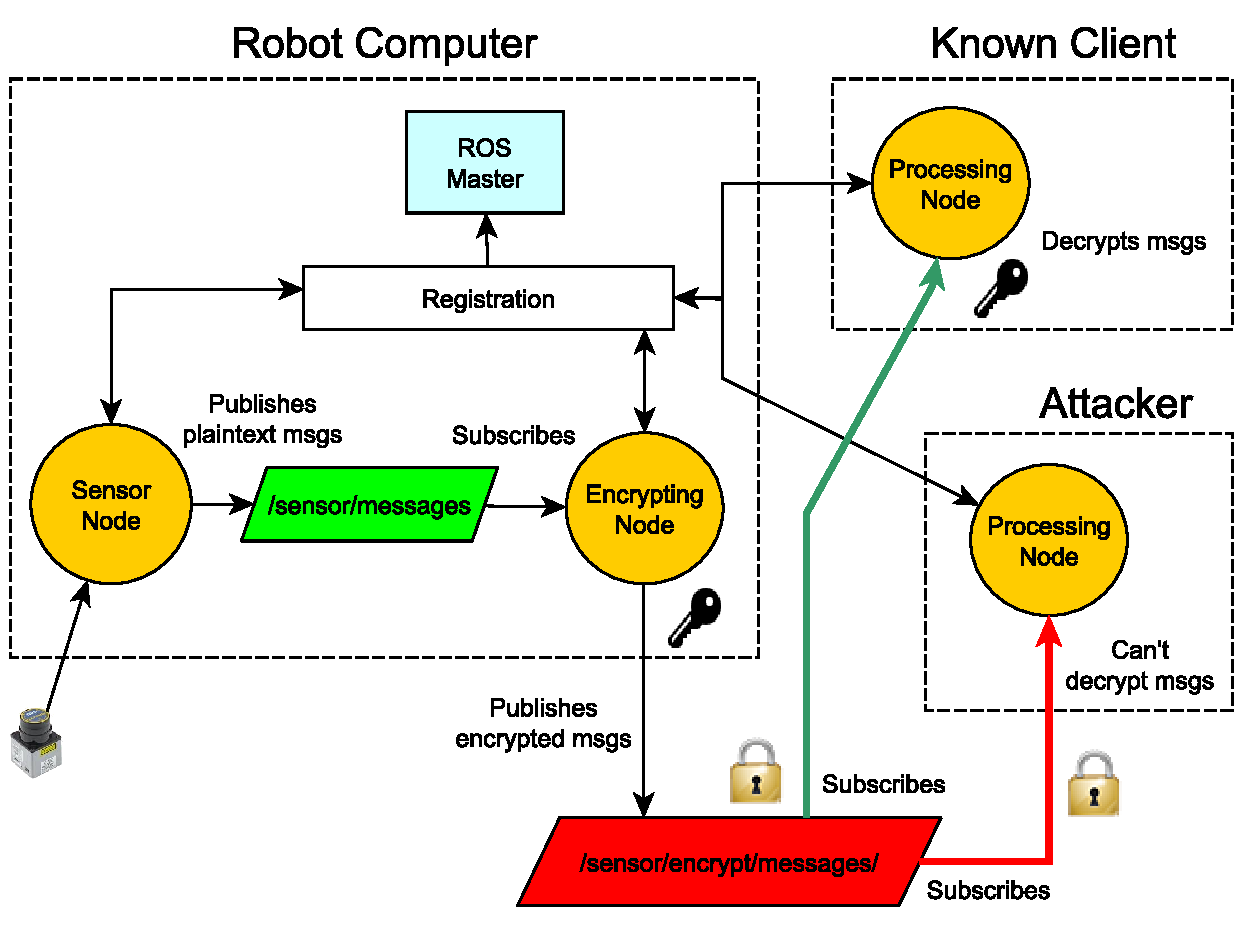
\includegraphics[width=.5\textwidth]{TestBed_complete.pdf}
	\caption{Scheme of the scenario used for testbed.}
	\label{fig:TestBed}
\end{figure}

%\textcolor{red}{TRADUCIR:} Un robot con un PC corriendo el master. Un sensor láser conectado al PC del robot. Un nodo de cifrado corriendo en el robot, que cifra los mensajes del láser y los publica en el topic "laser/encryted" (por ejemplo).
%Por otro lado, hay un PC cliente con ROS, que se registra en el master. Se suscribe al topic "laser/encryted" y como conoce la clave, es capaz de descifrar la información proporcionada por el láser.

First, we installed ROS Indigo in the on-board computer of the our RB1 mobile robot. The ROS master component ran in this platform. The robot was connected by wire to our laboratory network infrastructure. First we used the Hokuyo laser sensor of the robot. We launched a Hokuyo node that published laser data in the topic \textit{/laser}. Then, we ran {\textcolor{red}{our encryption node, antes hay que decir que nodos hay}} which subscribes to \textit{/laser}, performs data encryption and publishes them into \textit{/encrypted/laser} topic.

Second, we used one desktop computer as a ``known client'', also with ROS Indigo installed and connected by cable to our network. This client knows the master ROS IP, so it can communicate with master. We run a decryption node in the client computer, which registers to master and subscribes to the topic \textit{/encrypted/laser}. This node decrypts data and prints them on the screen.

Third, we used another desktop computer as a simulated ``attacker'', connected to the same  cable network. This computer has the same ROS version running on it. The attacker doesn't know the master ROS IP, but he can easily discover it performing a network scan with well known tools like \textit{nmap}. Then, the attacker could execute a malicious node for attempting to read laser data, which is being published in the topic \textit{/encrypted/laser}. Despite the node could subscribe to that topic, all data received is encrypted. As a result, the malicious node can't see original laser messages because the attacker doesn't have the key to decrypt them. 

%Al mismo tiempo, un atacante desde otro PC con ROS, intenta hacer lo mismo. Escanea la red hasta dar con la IP del master y se registra. Pero gracias a nuestra soluci\'on, aunque se suscriba al topic para obtener los datos del l\'aser, no es capaz de ver nada legible porque no conoce la clave de descifrado.

%\textcolor{red}{TRADUCIR:} Para las pruebas, la clave para cifrar/descifrar la tienen guardada tanto el master como el cliente conocido. En un sistema real, este proceso debería hacerse mediante un sistema de clave pública-privada como RSA, para transmitir de una forma segura la clave que van a compartir ambos nodos.

The cryptographic key  is stored in the master node and it is known by the legitimate clients. In a system in production this mechanism can be implemented as a public-private key schema as RSA  to safely share the key between the nodes. 


%In this case, two clients are connected to a topic. This situation is transparent to ROS Master.
%The standard process starts with a basic sensor node (BSN). We have defined as BSN those ROS nodes in charge of to publish the information from the sensor.
%We have prepared a testbed with two laptopts.




%We have installed ROS Indigo in two computers connected through a wired Ethernet 10/100 switch (model XXXX).
%In the first computer we connected an Asus Xtion camera and a Hokuyo laser sensor. The second computer was running a node for visualizing the sensors information sent by first computer. %Figure \ref{fig:maqueta} shows this environment.

% Then we modified the standard ROS implementation. We changed the TCP/IP sockets based implementation by ciphered ones.


\subsection{Encrypting ROS messages}

%%%  DESCRIBIR SISTEMA DE CIFRADO QUE USAMOS

% Decir que: SÓLO HEMOS AÑADIDO CIFRADO Y DESCIFRADO EN LOS NODOS EMISORES Y RECEPTORES. NO HEMOS MODIFICADO EL SISTEMA DE BAJO NIVEL DE ROS, PARA EVALUAR ESPECÍFICAMENTE Y DE UNA FORMA MÁS PRECISA LA CARGA QUE SUPONE EL CIFRADO EN LOS NODOS.

In this first approach we have changed the data published by the node, and instead of publish the information in a plain manner, we publish the information encrypted. 

ROS uses a {\em messages description language}\footnote{\url{http://wiki.ros.org/msg}} for describing the data values that each node publish. In this manner, it is easy for ROS tools to automatically generate source code for the message type in several target languages as ICE or idl. 

There are built-in types (14), array types (4) and customized types. For instance, if we get the {\em sensor\_msgs/Image.msg} message, we find a composed message by one non built-int message, and five built-in (3 x uint32, 1 x string, 1 x uint8 )and one array type (uint8[]).

{
	\footnotesize{
	\begin{Verbatim}[frame=single, commandchars=+\(\)]
std_msgs/Header header #custom msg

uint32 height
uint32 width
string encoding
uint8 is_bigendian
uint32 step

+underline(uint8[] data) #matrix data of an image
	\end{Verbatim}
	}
}

In this case is {\em data} field the element that contains the information of the image grabbed by the camera, so we are going to encrypt this element before to be publisher in ROS distributed system.



We use the 3DES algorithm to provide a security layer to ROS data.
It  is  a  known that  3DES cyphering speed is slower~\cite{singh2013study} than other cipher methods as for instance AES. As the worse environment, this is the motivation to analyze its behaviour in a real environment with ROS.
Triple DES (3DES) references the Triple Data Encryption Algorithm (TDEA or Triple DEA). It is a symmetric-key block cipher that applies the Data Encryption Standard (DES) algorithm three times to each data block. It is standardized by NIST in the Recommendation for the Triple Data Encryption Algorithm Block Cipher (NIST Special Publication 800-67).

DES algorithm has a fixed data block size of 8 bytes. Its keys are 128 (option 1) or 192 bits (option 2) long. However, 1 out of 8 bits is used for redundancy and do not contribute to security. The effective key length is respectively 112 or 168 bits.

The plaintext is first encrypted with K1, then decrypted with K2, and finally encrypted again with K3. The ciphertext is decrypted in the reverse manner.

The 192 bit key is a bundle of three 64 bit independent subkeys: K1, K2, and K3.

The 128 bit key is split into K1 and K2, whereas K1=K3.

It is important that all subkeys are different, otherwise 3DES would degrade to single DES.

3DES is cryptographically secure, although it is slower than AES algorithm. In a next stage, we will substitute 3DES with AES in our encryption system and repeat all the test we have done, to compare the performance.


From the development side, tt was used the PyCrypto package. It is an extended python Cryptography Toolkit that allows to simply the method to encrypt or decrypt in multiple languages. 



\section{Experimental Measurements}
\label{experiments}
%\textcolor{red}{COMENTAR A ALTO NIVEL QU\'E/CU\'ANTAS PRUEBAS HEMOS HECHO.}

To illustrate the described approach, we present an ad-hoc implementation of an encryption system to change part of the message used for transmit or receive robot sensors information. 
We maintain in each case 

% Figure \ref{fig:velocidad-maqueta} shows the maximum rate that can be reached both in the laser and the camera visualization according to \texttt{rviz} information.

The same measurements were made in the second environment to see whether the use of wireless systems and a real robot have any impact.

% The absolute values of the frame rates is obviously different, as shown in figure \ref{fig:velocidad-robot}. But the interesting part is the relative different when using clear communications or ciphered ones. 

% Table \ref{tab:relativas}  compares the relative reduction of speed when using ciphered protocols vs clear ones in both environments as well as the relative increase of CPU usage.

%The decorator pattern can be used to extend (decorate) the functionality of a certain object statically, or in some cases at run-time, independently of other instances of the same class, provided some groundwork is done at design time. 
We have added a function to our program in order to measure the time spent on each encryption and decryption call. The function is a python method presented as a decorator pattern, which is used here to extend the functionality of encryption/decryption at run-time. 


{
  \footnotesize{
    \begin{Verbatim}[frame=single]
def fn_timer(function):
	  @wraps(function)
	  def function_timer(*args, **kwargs):
	      v_time_0 = time.time()
	      result = function(*args, **kwargs)
	      v_time_1 = time.time()
	      return result
	  return function_timer
    \end{Verbatim}
  }
}

We have divided the experiments in three parts. First we have analyzed how does the "Publisher-listener"  ROS nodes work under encrypted conditions. Then we have stressed the same nodes publishing bigger text messages, in plain text as well as encrypted text. Finally we have analyzed a camera sensor, under the same encryption/decryption conditions.  

\subsection{Hardware/Software Set-up}



We want to evaluate how the encryption of communications would affect the performance of ROS.
We have used the better of the cases where a 8x Intel(R) Core(TM) i7-4790 CPU @ 3.60GHz
with 16231MB of RAM Memory	and running an Ubuntu 14.04.4 LTS Operating System.
The ROS master system has 234 process running by default, the client is running 242 process.

The two computers are connected by an  Alcatel-Lucent OmniSwitch 6860E switch
This hardware conditions are the most favorable against the real environment of a robotic platform for instance wireless or hardware restrictions.


\subsection{Test 1: HelloWorld Publisher-Listener Node}

In this test we have used the version of talker/listener tutorial proposed by ROS\footnote{\url{http://wiki.ros.org/rospy_tutorials/Tutorials/WritingPublisherSubscriber}}

This package distributed by ROS as a demo, presents a simple ROS package that creates two rospy nodes. The "talker" node broadcasts a {\em Hellow world + Timestamp} message on topic "chatter", while the "listener" node receives and prints the message.


%======================================
%Cifrado
%======================================
%Cifrado length: 1272.000000
%Cifrado min: 0.000040
%Cifrado max: 0.000129
%Cifrado mean: 0.000065
%Cifrado stdev: 0.000000
%El valor moda de la fase de cifrado fue:
%(array([  4.60147858e-05]), array([ 55.]))
%======================================
%Descifrado
%======================================
%Cifrado length: 1570.000000
%Cifrado min: 0.000023
%Cifrado max: 0.000239
%Cifrado mean: 0.000045
%Cifrado stdev: 0.000000
%El valor moda de la fase de cifrado fue:
%(array([  4.50611115e-05]), array([ 260.]))
\begin{table}[h]
	\centering
	\caption{Time in seconds of CPU spent on a simple publisher/listener running test.}
	\label{tab:time_simple_text_hellow_CPU}
	\begin{tabular}{|l|l|l|l|l|}
		\hline
		&		Plain&	Plain&	Encrypt&	Decrypt \\
		&		Publication&Subscription&Publication&Subscription \\\hline
		Time running&34.491&	34.484&	36.882&	34.995 \\\hline
		Time user&0.184&	0.196&	0.348&	0.24 \\\hline
		Time sys&0.024&	0.08&	0.064&	0.056 \\\hline
		Total CPU&0.208&	0.276&	0.412&	0.296 \\\hline
		
	\end{tabular}
\end{table}

Table~\ref{tab:time_simple_text_hellow_CPU} presents the CPU time spent when the nodes are running in different machines.  The values are the result of launching ROS nodes using the Unix command {\em time}. The values present a minimal consumption of CPU associated to the process. In  case of Plain publish/subscribe it represents than 1\% and in the case of the publisher in encrypt mode it represents approximately the 1.1\%, that is almost the same than in plain mode.

%\begin{figure}[ht!]
%	\centering
%	\includegraphics[width=.5\textwidth]{Text_plain_vs_encrypted.png}
%	\caption{Time of CPU spent on a simple publisher/listener 30 seconds running test.}
%	\label{fig:time_simple_text_hellow_CPU}
%\end{figure}

\begin{figure}[ht]
	\centering
	\includegraphics[width=.5\textwidth]{figure_Simple_Publisher_subscriber1.png}
	\caption{Histogram showing the time spent on a encrypt/decrypt DES3 function call.}
	\label{fig:time_simple_text_CPU}
\end{figure}

\begin{figure*}[ht!]
	\centering
	\includegraphics[width=.99\textwidth]{Screenshot_hello_world.png}
	\caption{Screen-shot with the nodes involved in the simple publisher/subscribe test. Upper left terminal presents the publisher node before encryption. Bottom left terminal depicts the subscriber node after decryption. Right terminal presents the results of rostopic echo on {\em /chatter} topic used for transmitting info through nodes.}
	\label{fig:screenshot_hello_world}
\end{figure*}


Figure~\ref{fig:time_simple_text_CPU} presents the histogram associated to the calls to encrypt/decrypt method used in these tests.  We can observe that the average time in the encryption process is slightly higher (0.000065 seconds) than the decryption process (0.000045 second). However, in both cases it is almost negligible. The worst case presented a 0.000129 seconds in ciphering time and  0.000239 second of deciphering time.


Figure~\ref{fig:screenshot_hello_world} presents the screenshot of this experiment. It shows the three terminals from the two nodes involved in this experiment. Publisher node (top-left window) that presents a simple log, subscriber node with key (bottom-left) that presents the message after the decryption call and subscriber node without key ({\em rostopic echo }) that shows the encrypted message in the topic.


\subsection{Test 2: Custom Text Publisher-Listener Node}


In this test we have used the same version of talker/listener nodes proposed by ROS. In this particular test we generate a sintetic text strings with different sizes:
\begin{itemize}
\item T1: this is a string message of 262144 bytes (256 KB)
\item T2: it is a string message of 524288 bytes (512 KB)
\item T3: presents a string message of 1048576 bytes (1024 KB)
\end{itemize}  


We want to determine the duration of execution of our talker and the time spent by our listener nodes. Again, we run the Linux {\em time} command to measure the total CPU time consumed by the ROS talker process. 

Initially we run the test with the three size types of messages using plain text. 
We have performed the test three times, running the nodes for a time lapse of 30 to 35 seconds. 
Firstly, reviewing the  T1 type (it is presented in a time window of 32.884 seconds) we find   a CPU time of 1.408 seconds. It was a user time of  1.364 seconds and a sys time of 0.044s. I
Secondly, we analyse the string of type T2. It was launched in a  window of 33.749 seconds, and needed a total CPU of a  2.672 seconds (user time of 2.508 seconds and a sys time of 0.164s). 
Finally, we analyse T3, that presents in a time window of 34.731 seconds a total CPU of 5.260 seconds (it is divided by a user time of  5.140 seconds and a sys time of 0.120s).

\begin{figure}[ht!]
	%    \centering
	\includegraphics[width=.5\textwidth]{Figura_t1t2t3.png}
	\caption{Time of CPU spent by publiser/subscriber nodes sending T1, T2 and T3 messages in plain and Encrypted/Decrypted on test 2.}
	\label{fig:time_text_CPU}
\end{figure}

This is totally different when we are working with encrypted text messages. Fig~\ref{fig:time_text_CPU} presents the main differences. We have repeated the same experiment, but this time calling an encryption method that encrypts from plain text to 3DES. It is possible to see that the encrypt process consumes more CPU than  the plain process.
For instance, T1 type presents running for 34.486 seconds a total of 23.008 of CPU. This means that the total CPU time increases almost 62\%. This is even higher in T2 and T3 types with almost the 98\% of real execution time. It is clear that the encrypted/decrypted approach consumes more CPU (yellow bars in Fig.~\ref{fig:time_text_CPU}) than plain text (orange bars in Fig.~\ref{fig:time_text_CPU}). 



\begin{figure}[ht]
	\centering
	\includegraphics[width=.5\textwidth]{Outline_images_encryption_decrytiontime4.png}
	\caption{Histogram by each publisher node attending each call to the encryption method.}
	\label{fig:text_encryption_time}
\end{figure}

%\textcolor{red}{[REESCRIBIR BIEN ESTE P\'ARRAFO].} 
We know that the encryption process needs more CPU, but how long does the process of encryption/decryption take in each block?. Just for clarification, we review the encryption phase in the publisher node.
In case of T1 messages, during its window (34.486s) the node is able to encrypt 1040 messages. The minimal time to perform this task is 0.059246 seconds and the maximum time to encrypt the string is 0.683408 seconds. In average, the system spents 0.063858 seconds (standard deviation of 0.000388 seconds).
This time increases with T2 and T3 types. T2 type needs 0.123383 seconds in average with standard deviation of 0.000040 seconds and  T3  0.247303 with a standard deviation of 0.000137.
Fig.~\ref{fig:text_encryption_time} presents the histogram associated to this experiment.



% raspberry@david-H97M-D3H:~/catkin_ws/src/security_repo/ciphering_project/simple_talker_listener/src$ time python talker3DES.py
% ;;;;;;;;
% ^C
% real    0m34.486s
% user    0m22.924s
% sys    0m0.084s
% raspberry@david-H97M-D3H:~/catkin_ws/src/security_repo/ciphering_project/simple_talker_listener/src$ time python talker3DES.py
% ;;;;;;;;
% ^C
% real    0m40.607s
% user    0m40.368s
% sys    0m0.232s
% raspberry@david-H97M-D3H:~/catkin_ws/src/security_repo/ciphering_project/simple_talker_listener/src$ time python talker3DES.py
% ;;;;;;;;
% ^C
% real    0m38.718s
% user    0m38.416s
% sys    0m0.248s



% where 0m34.731s of execution 
% user    0m5.140s
% sys    0m0.120s
% 
% raspberry@david-H97M-D3H:~/catkin_ws/src/security_repo/ciphering_project/simple_talker_listener/src$ time python talker.py
% ^C
% real    0m33.749s
% user    0m2.508s
% sys    0m0.164s
% 
% raspberry@david-H97M-D3H:~/catkin_ws/src/security_repo/ciphering_project/simple_talker_listener/src$ time python talker.py
% ^C
% real    0m32.884s
% user    0m1.364s
% sys    0m0.044s
% ======================================
% 256
% ======================================
% Cifrado length: 1040.000000
% Cifrado min: 0.059246
% Cifrado max: 0.683408
% Cifrado mean: 0.063858
% Cifrado stdev: 0.000388
% El valor moda de la fase de cifrado fue:
% (array([ 0.06053495]), array([ 3.]))
% ======================================
% 512
% ======================================
% Cifrado length: 309.000000
% Cifrado min: 0.120618
% Cifrado max: 0.229785
% Cifrado mean: 0.123383
% Cifrado stdev: 0.000040
% El valor moda de la fase de cifrado fue:
% (array([ 0.12165689]), array([ 2.]))
% ======================================
% 1024
% ======================================
% Descifrado length: 147.000000
% Descifrado min: 0.242966
% Descifrado max: 0.386008
% Descifrado mean: 0.247303
% Descifrado stdev: 0.000137
% El valor moda de la fase de descifrado fue:
% (array([ 0.24460196]), array([ 2.]))



\subsection{Test 3: Camera Node}


%\subsubsection{Process evaluation}
The third experiment has been developed using a RGB camera. A Logitech, Inc. QuickCam Pro 9000 webcam will provide a frame rate of 15 fps @ 640x480 of resolution. This sensor will be registered on ROS system to provide images to the environment.

This test involves three ROS nodes, two from the publisher side: usb\_cam, encrypted\_node and one from the listener side: decrypted\_node. First ROS node,{\em usb\_cam}\footnote{\url{http://wiki.ros.org/usb_cam}} is developed by Benjamin Pitzer and still maintained by ROS developers. It is in charge of to grab information from sensor and publish in a topic.
The second node runs in the same computer and it is in charge of encrypt the message published by {\em usb\_cam}. The third node runs on the second computer, it is in charge of decrypt the messages distributed by publisher node and to display the original image on display.
\begin{figure*}[ht!]
	\centering
	\includegraphics[width=.99\textwidth]{Screenshot.png}
	\caption{Screenshot taken during image encryption test.}
	\label{fig:screenshot}
\end{figure*}



Figure \ref{fig:screenshot} presents the situation in a given moment $T$ on the listener node. We have used the ROS node {\em image\_view} to visualize the images from topics.  There is an non-encrypted topic that we have maintained in order to validate delays. There is an encrypted topic that is not possible to visualize using the released image\_view ROS node. Finally there is a frame that presents the image after decrypt the topic using our own decrypt node. 

%There are three topics involved: \textcolor{red}{[COMPLETAR]}


Again, we measure the time needed to encrypt or decrypt the ROS message ({\em sensor\_msgs/Image.msg}). We just encrypt or decrypt the field data of {\em uint8[]} that is treated as a string. To evaluate  the frame rate, our nodes present this information during the execution in the visualization frame . 

This experiment was running for about 18 hours sending in total 971790 frames. The average time in the process of encrypt the sensor data was 0.010948 seconds (stddev 0.000004s).
Minimal procesing time was 0.001309 seconds and max procesing time was 0.026909 seconds. 
%mean of  0.010948 seconds and a standard deviation of 0.000004 seconds. The mode value in this phase was 0.010571 seconds wich was reapeated 415 times. 
The average time to decrypt the images was 0.008828 seconds (stddev 0.000003s).
The max time decrypting an image was 0.039130s and the minimal 0.001288s. 
%%The minimal time to decrypt the images was 0.001288 seconds, the max time was 0.039130 seconds with a mean of  0.008828 seconds and a standard deviation of 0.000003 seconds. The mode value in this phase was 0.008183 seconds wich was reapeated 593 times. 





\begin{figure*}[ht!]
	\centering
	\includegraphics[width=.99\textwidth]{Outline_images_encryption_decrytiontime2.png}
	\caption{Time spent on each call to encryption/decryption function during the image processing in test 3.}
	\label{fig:images_encryption}
\end{figure*}


\section{Discussion}

This  study  provides  an  in-depth  characterization  of  the  3DES encryption under most positive conditions. On the one hand, we have two nodes ready for high performance due its  hardware characteristics.  On the other hand, the software on both machines is limited to those nodes needed for the test, no extra computational process are launched.

Results presented in first test, showed than there is no difference between to send a simple plain string of chars {\em Hello world + timestamps}  and a encrypted string of chars. 
However, these data do no support the possibility of continuously  use encrypted methods. Total CPU time consumed by publisher node when the string increases to 256KB suggest that this situation can decreases overall system performance.    

ROS provides a statistical data system that shows the publish/subscribe performance between 
connected nodes. When the system is active on a node, the statistical data is published in a new topic updated each second .%({\em std\_msgs/String})

Under these conditions, we have observed two main issues: the first related with traffic and the second related with the number of delivered messages. The first issue imply that the traffic in bytes increases under the same conditions of speed (delivered messages) For instance when the test 1 is running, during one second: 
\begin{enumerate}
	\item plain mode presents  10 messages  with 346 bytes of traffic (in average).
	\item encrypted mode presents 10 messages in average with 420 bytes of traffic (in average).
\end{enumerate}

The second issues comes, under higher peformance requirements as in test 2, sending messages of type T3. In a second we can find:
\begin{enumerate}
	\item plain mode presents  10 messages  with 11010132 bytes of traffic (in average).
	\item encrypted mode presents 5 messages in average with 5242880 bytes of traffic (in average).
\end{enumerate}



%Descifrado length: 285.000000
%Descifrado min: 0.234246
%Descifrado max: 0.273480
%Descifrado mean: 0.240323
%Descifrado stdev: 0.000021
%El valor moda de la fase de descifrado fue:
%(array([ 0.23816991]), array([ 2.]))

Under these conditions the number of messages per second is reduced to the half. There are one main reason  to get these results, publisher node needs at least 0.247303 seconds to encrypt the message and the listener node also needs 0.240323 with a stddev 0.000021. The situation is even worst when the listener also has to do something with the message. For instance just printing the message on the screen reduce the overall performance to 2 messages per second. 

%
%times presented by our test2 presents  sending 11 string messages  per second (with ``Hello wold'' text), plus a timestamp with 440 bytes of traffic.
%In this manner, we wanted to analyse the behaviour of the system using bigger messages:
%
%The behaviour of ROS traffic using  with simple plain messages {\em delivered\_msgs} 10 of T1 generate . When T2 messages are sent the system runs with 4194368 bytes of traffic and finally when it is working in  T3 messages just send 4194336 bytes and a total of 4 messages. There is no dropped messages by subscription.

Finally, the experimental procedure follow in test 3 does not show a significant delay produced by encryption, it means that under these condition it does not reduce the camera frame rate. The FPS in the publisher machine was 14.56 and the FPS in the decryption machine was 14.54.



Fig.~\ref{fig:images_encryption} outlines the behaviour of the publisher cyphering data. Left part of the figure presents the box plot of the three types of message. The right part of the element present the histogram associated to the time in each call to the encryption method. We observe close processing times (in average) in the encryption/decryption process similar to other researchers results\cite{elminaam2008performance}. {\color{red}{deberíamos decir algo bonito aqui}.}


%
%
%The figure~\ref{fig:images_encryption} presents the box-plot of the encryption decryption data analyzed and the histograma. 

%rosparam set enable\_statistics true





% % % % % % % % % % % % % % % % % % % % % % % % % % % % % % % % % 
%  Camara
% *****************************************************
% load avg
% *****************************************************
% 1m
% Cifrado length: 73583.000000
% Cifrado min: 0.000000
% Cifrado max: 4.090000
% Cifrado mean: 0.420771
% Cifrado stdev: 0.402261
% El valor moda del elemento 1m: (array([ 0.01]), array([ 2720.]))
% 5m
% Cifrado length: 73583.000000
% Cifrado min: 0.070000
% Cifrado max: 1.330000
% Cifrado mean: 0.420862
% Cifrado stdev: 0.062276
% El valor moda del elemento 5m: (array([ 0.27]), array([ 2261.]))
% 15m
% Cifrado length: 73583.000000
% Cifrado min: 0.190000
% Cifrado max: 0.710000
% Cifrado mean: 0.420539
% Cifrado stdev: 0.009572
% El valor moda del elemento 15m: (array([ 0.39]), array([ 3407.]))
% 
% 
% 
% *****************************************************
% net/eth0
% *****************************************************
% recv
% Cifrado length: 73583.000000
% Cifrado min: 0.000000
% Cifrado max: 2894889.000000
% Cifrado mean: 180.865336
% Cifrado stdev: 152873314.363260
% El valor moda del elemento recv: (array([ 0.]), array([ 39574.]))
% send
% Cifrado length: 73583.000000
% Cifrado min: 0.000000
% Cifrado max: 16727.000000
% Cifrado mean: 0.987021
% Cifrado stdev: 9843.397769
% El valor moda del elemento send: (array([ 0.]), array([ 73511.]))
% 
% % % % % % % % % % % % % % % % % % % % % % % % % % % % % % % % % 
% Idle PC
% % % % % % % % % % % % % % % % % % % % % % % % % % % % % % % % % 

% *****************************************************
% net/eth0
% *****************************************************
% recv
% Cifrado length: 73950.000000
% Cifrado min: 0.000000
% Cifrado max: 2429716.000000
% Cifrado mean: 199.616822
% Cifrado stdev: 134166979.708237
% El valor moda del elemento recv: (array([ 0.]), array([ 34878.]))
% send
% Cifrado length: 73950.000000
% Cifrado min: 0.000000
% Cifrado max: 14811.000000
% Cifrado mean: 23.408343
% Cifrado stdev: 12934.495778
% El valor moda del elemento send: (array([ 0.]), array([ 64845.]))
% 
% *****************************************************
% load avg
% *****************************************************
% 1m
% Cifrado length: 73950.000000
% Cifrado min: 0.000000
% Cifrado max: 4.520000
% Cifrado mean: 0.310385
% Cifrado stdev: 0.599820
% El valor moda del elemento 1m: (array([ 0.]), array([ 41293.]))
% 5m
% Cifrado length: 73950.000000
% Cifrado min: 0.020000
% Cifrado max: 1.360000
% Cifrado mean: 0.311375
% Cifrado stdev: 0.094693
% El valor moda del elemento 5m: (array([ 0.04]), array([ 5726.]))
% 15m
% Cifrado length: 73950.000000
% Cifrado min: 0.130000
% Cifrado max: 0.620000
% Cifrado mean: 0.311785
% Cifrado stdev: 0.012632
% El valor moda del elemento 15m: (array([ 0.22]), array([ 3330.]))



\section{Conclusion and Further Work}
\label{conclusions}
This article has introduced the use of encrypted information through ROS communication system.
We have evaluated the impact of this added feature from two points of view: CPU consuming and network traffic. 

We have shown that our approach avoids security problems related with the plain-text publish/subscribe paradigm used by ROS. However, the overhead of CPU performance and communication load should also be considered in distributed architectures that need to work on real time.

As we pointed out in the introduction, securing communications is just one dimension in the cybersecurity of autonomous systems. If we want to see these machines working in our homes we need to secure navigation abilities and interaction mechanisms, to avoid manipulated or malicious behaviours and make robots reliable assistants for every person at home.


\section*{Acknowledgment}
The authors would like to thank the Spanish Ministry of Economy and Competitiveness for the partial support to this work under grant DPI2013-40534-R and to the Spanish National Institue of CyberSecurity (INCIBE) under grand Adenda21 ULE-INCIBE.

\bibliographystyle{plain} 
\bibliography{waf2016}

\end{document}

